\section{Research process}
\subsection{Starting out: Levenshtein with dynamic programming}
For a start, a naive version of the Levenshtein distance metric was
implemented, but as expected, this is absolutely useless in any practical
setting, since it does not reuse already calculated results. Therefore, this
was quickly transformed into a dynamic programming solution, which solves
subproblems just once, stores and reuses the intermediate results. This dynamic
programming bottom up solution was however still very slow, yielding a
performance of around 70 comparisons per second. This could most likely be
optimized further, but because of the characteristics of an edit distance
algorithm like Levenshtein and because of the performance requirements for this
project, we choose to not pursue further optimization and instead focus on
other types of algorithms.

\subsection{Simple $d2$ distance}
After learning that the basic Levenshtein algorithm is far too slow for the
problem domain of this project, we turned our attention to the $d2$ distance
metric. The first version of the $d2$ distance metric algorithm is shown in
figure \ref{alg:d2_naive}. This algorithm maintains a single frequency vector,
as a map structure to allow for large $k$ which results in a large number of
possible different $k$-mers. The map is indexed using the lexicographical
position of the $k$-mer. When iterating through the first sequence, $k$-mer
counts are incremented and when iterating through the second sequence, they are
decremented. Finally all the frequencies are squared and the square root of the
sum is returned, corresponding to the Euclidean distance between frequency
vectors for the two sequences.

\begin{algorithm}
  \caption{Naive \textsc{d2} distance metric}
  \label{alg:d2_naive}
  \begin{algorithmic}[1]
    \Require{$s$ and $t$ are DNA or RNA sequences and $k \in \mathbb{Z}^+$}
    \Statex
    \Function{d2}{$s, t, k$}
      \State initialize \texttt{freq\_map}
      \For{$i \gets 0$ to $length(s) - k$}
        \State freq\_map[index\_of\_kmer(s.substring(i, k)]\texttt{++}
      \EndFor
      \For{$i \gets 0$ to $length(t) - k$}
        \State freq\_map[index\_of\_kmer(t.substring(i, k)]\texttt{--}
      \EndFor
      \State $total \gets 0$
      \ForAll{$e \in$ freq\_map}
        \State $total \gets e.value^2$  \Comment{calculate the Euclidean distance}
      \EndFor
      \State \Return $\sqrt{total}$
    \EndFunction
  \end{algorithmic}
\end{algorithm}


\subsection{$d2$ distance with windows and Jaccard index}
The current version of the $d2$ distance function uses the concept of a
\emph{window}, of a certain length, that iterates over the sequences and
calculates distances between the substrings in each window. This calculation is
done using a kind of forward differences method for reducing the calculations
to a few fixed operations for calculating the distance in the next window from
the distance in the current window. This concept is described in
\cite{hazelhurst}.

The algorithm presented here uses a window size equal to the length of the
shortest of the two sequences. Let $|s|$ be the length of the shortest of the
two sequences. To begin with the, the $k$-mers in the first $|s|$ characters of
each sequence are counted and the \emph{Manhattan} distance between these two
frequency vectors is calculated.

The Manhattan distance is simply the Euclidean distance where squaring is
replaced with absolute value and the square root is omitted, i.e. for
$u, v \in \mathbb{Z}^n$, 
\begin{equation}
  d_{Manhattan} \eqdef \sum_{i=1}^{n} |u_i - v_i| \;.
\end{equation}

This distance is the distance between the subsequences in the first position of
the window. To calculate the distance in the following window, i.e. advancing
the window through the longer of the two sequences by one character, it is
decided which $k$-mers exit and enter the window, respectively, and then by
looking at whether the existing $k$-mer count in the frequency vector is
negative or positive, it can be decided whether the distance increases or
decreased by 2 or whether it stays the same. Subsequently, the frequency vector
is updated to reflect the change in the new window. The following illustrates
the idea of a window and $k$-mers exiting and entering the window:
\begin{verbatim}
      |---- window ----------|
      ACTGATCGTAGCTAGCTAGTGTTG
      ACGTAGATCGTGGATGGCTGATCGTAGCTAAGCTTAGCTGATCG.....
      ^^^^                 ^^^^
      k-mer exiting        k-mer entering
\end{verbatim}

Since the Manhattan distance can be hard to use in practice, since it is very
dependent on the length of the shortest sequence (the length of the window),
the concept of the \emph{Jaccard index}, or the \emph{Jaccard similarity
coefficient}, is used to ``normalize'' the distance to a value in the interval
$[0,1]$.

The Jaccard index of two sets $A$ and $B$ is defined as follows:
\begin{equation}
  J(A, B) \eqdef \frac{|A \cup B| - |A \cap B|}{|A \cup B|}
\end{equation}
 % TODO:  maybe actually Jaccard distance; maybe add citation

In the context of $k$-mer frequencies, the union can be interpreted as the
total number of $k$-mers in the window in the two sequences, and the
intersection as the Manhattan distance in the window.


\subsection{Evaluating distance metric}
To evaluate our implementation of the $k$-mer distance using windows and
Jaccard index, we decided to use the Levenshtein distance as reference.\\ Since
Levenshtein distance does not produce values between $0$ and $1$, we have
normalized it so it uses Jaccard index.

In figure \ref{fig:Levenshtein_vs_Kmer} is three scatter plots with the
Levenshtein distance on the $y$-axis and our version of the $k$-mer distance on
the $x$-axis. The three plots are with $k=4, k=6$ and $k=8$.

The scatter plots gives an indication about when and how sensitive our
implemented distance metric is. We want the distance to be as close as possible
to a linear function without too much variance, but not necessarily to the line
$y=x$. If it can be expressed linearly it means there is a correlation between
the two. If it can be expressed as $y=x$ (or close) it means that they measure
the same distance which is favourable.

When $k=4$ there is a linear relation when the identity $I>0.9$, but when
$I<0.9$ there is too much variance in the points from any linear function.

With $k=6$ there seems to be a linear relation when $I>0.8$. When $I<0.8$ there
is more variance though less than when $k=4$.

When $k=8$, it is very similar to $k=6$. It seems there is a linear relation
for $I>0.8$ again and when $I<0.8$ the variance is greater.

\begin{figure}
        \begin{subfigure}[b]{0.5\textwidth}
        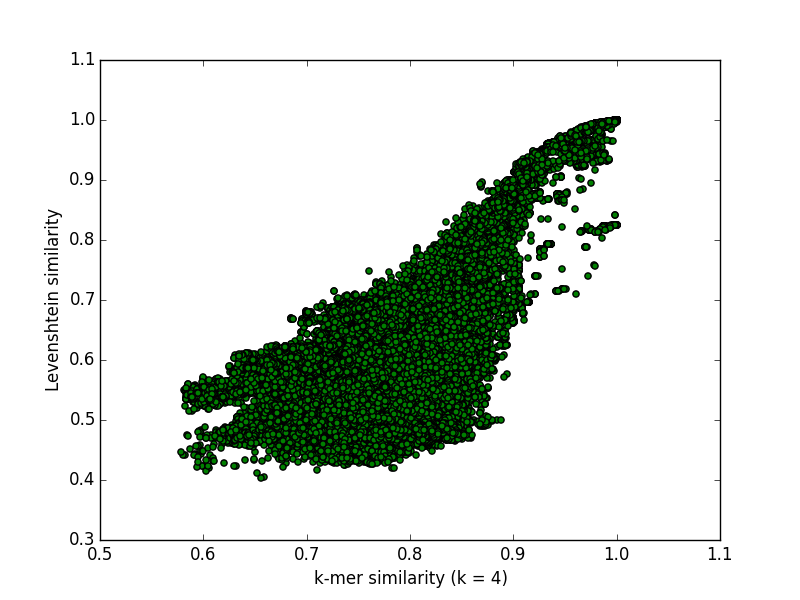
\includegraphics[scale=0.34]{graphics/k4.png}
        \end{subfigure}
        \begin{subfigure}[b]{0.5\textwidth}
        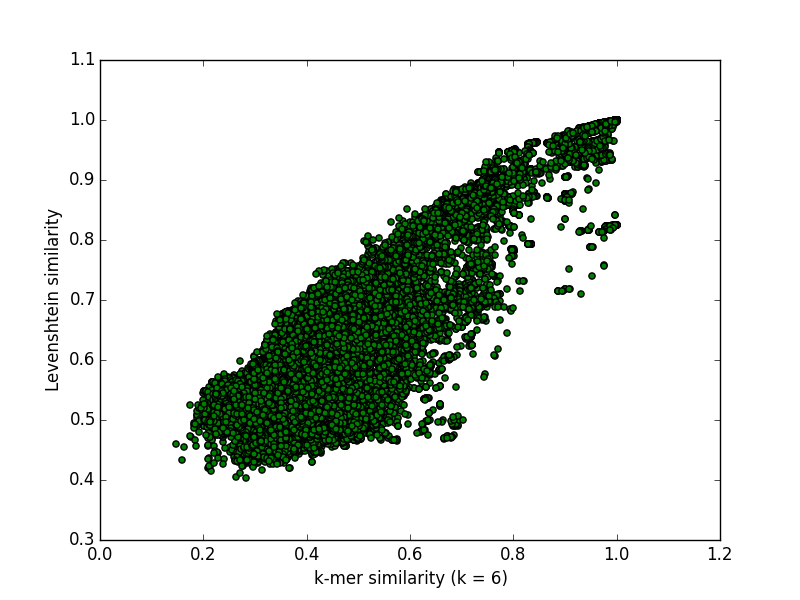
\includegraphics[scale=0.34]{graphics/k6.png}
        \end{subfigure}

  \centering
        \begin{subfigure}[b]{0.5\textwidth}
        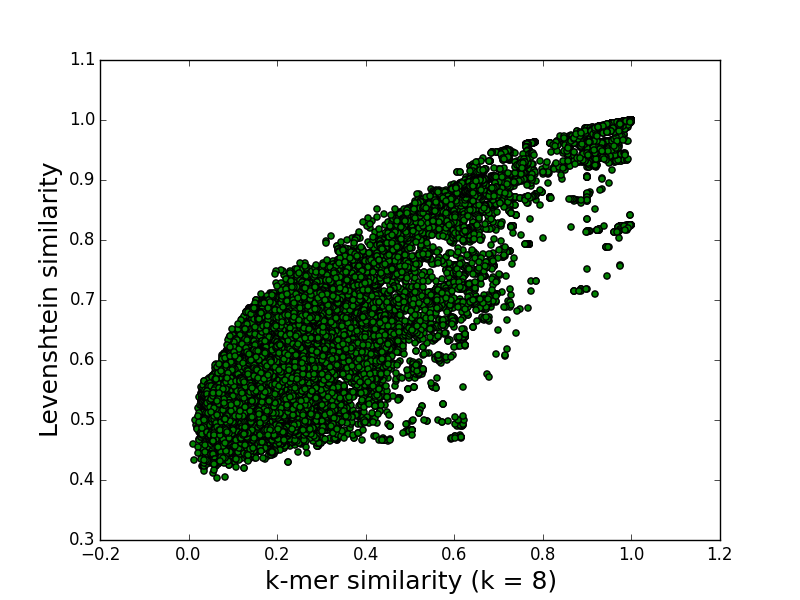
\includegraphics[scale=0.34]{graphics/k8.png}
        \end{subfigure}
\caption{Comparison of Levenshtein distance and our implementation of the
$k$-mer distance using windows and Jaccard index.}
\label{fig:Levenshtein_vs_Kmer}
\end{figure}


\subsection{Naive, greedy clustering algorithm} % TODO
% \item Implementing very (almost naively) greedy clustering algorithm.
Description and evaluation of a naive, greedy clustering algorithm which
compares every sequence to every centroid, found so far, until a match is found
and if not, the sequence becomes a new centroid. This running time of this
algorithm depends on the number of clusters in the output and therefore it
might be around $O(c^2)$, where $c$ denoted the number of sequences, in the
worst case where the number of clusters is equal to the number of sequences.  %O(k*(k-1)/2)


\subsection{\textsc{Simple\_Clust} algorithm}
We have developed a clustering algorithm, named \textsc{Simple\_Clust}
(Algorithm \ref{alg:simple_clust}), which will be described in this section.
\textsc{Simple\_Clust} works by iterating sequentially through the sequences to
be clustered; the $max\_reject$ most frequent $k$-mers for the query sequence
are calculated and for each of these most frequent $k$-mers, a centroid which
has that $k$-mer as the most frequently occurring one (if one such centroid
exists) is compared with the query sequence to check if distance is within the
given threshold. The query sequence is assigned to the cluster for the first
centroid that matches the query sequence; if no such centroid is found, out of
the maximum possible $max\_reject$ number of tries, the query sequence becomes
a centroid for a new cluster, the most frequent $k$-mer is decided and the
sequence, along with this information, is added to the collection of centroids.

This is repeated for all sequences in the input file.

\begin{algorithm}
  \caption{\textsc{Simple\_Clust}}
  \label{alg:d2_naive}
  \begin{algorithmic}[1]
    \Require{$S$ is an array of [DR]NA sequences, $k \in \mathbb{Z}^+$ and
             $max\_rejects \in \mathbb{Z}^+$, $id \in [0,1]$}
    \Statex
    \Function{Simple\_Clust}{$S, k, max\_rejects$}
      \State $cluster\_count \gets 0$
      \State $centroids \gets []$ \Comment{map from $k$-mer to sequence}
      \ForAll{$s \in S$}
        \State $mfk \gets$ $max\_rejects$ most frequent $k$-mers in $s$
        \ForAll{$m \in mfk$}
          \If{$centroids[m]$ does not exists}
            \State continue
          \ElsIf{$distance(s, centroids[m]) \geq id$}
            \State add $s$ to cluster with centroid $centroids[m]$
            \State write cluster output file
            \State break
          \EndIf
        \EndFor
        \If{matching centroid was not found}
          \State centroids.insert(mfk[0], s)
          \State write centroids output file
        \EndIf
      \EndFor
      \State \Return $cluster\_count$
    \EndFunction
  \end{algorithmic}
  \label{alg:simple_clust}
\end{algorithm}


\subsection{Comparing with UCLUST on real life data}
% Testing USEARCH 32-bit on real data
% Testing clustering algorithm with d2 distance and comparing performance to
% USEARCH.
Running \texttt{USEARCH} on the file \texttt{SILVA\_119\_SSURef\_tax\_silva.fasta} after it is sorted with parameters \texttt{-clust\_smallmem} and \texttt{-id 0.95} produces the following output

\begin{lstlisting}
28:39 1.1Gb  100.0\% 117205 clusters, max size 83904, avg 13.5                                                        
      Seqs  1583830 (1.6M)
  Clusters  117205 (117.2k)
  Max size  83904 (83.9k)
  Avg size  13.5
  Min size  1
Singletons  67410 (67.4k), 4.3\% of seqs, 57.5\% of clusters
   Max mem  1.1Gb
      Time  28:41
Throughput  920.3 seqs/sec.
\end{lstlisting}
While running our implementation of the same file but unsorted and with \texttt{id=0.9, k=6} og \texttt{max\_rejects=8} produces the following
\begin{lstlisting}
Reading 1583830 sequences...
Finished reading:
Time: 24.8109 sec.
Seqs/sec: 63836
Clustering 1583830 sequences...
26.4602
# of clusters: 1364006
Finished clustering:
Time: 187.355 sec.
Throughput: 8453.63seqs/sec.
\end{lstlisting}
Even though the \texttt{id}'s does not represent the same threshold due to it 
being two different distance metrics we do get a lot more clusters. Running 
it with similar \texttt{id}'s produces almost the same amount of clusters, so 
the problem lies in the way we choose our centroids we compare a query 
sequence with.

Our implementation, however, is faster by a factor of $10$. This can be 
attributed to our choice of distance metric.
\\
%Possibly things to look into: confusion matrix, Rand index, normalized
%mutual information (article: Comparing Clusterings - An Overview).


\subsection{Results}
\begin{figure}[H]
  \centering
  \begin{tabular}{ c | c }
    Metric                                        & Comparisons/second      \\
    \hline \hline
    Dynamic programming (bottom up) Levenshtein   & $\sim$ 70               \\
    \hline
    d2-distance with window, $k=4$                & $\sim$ 73000            \\
    \hline
    d2-distance with window, $k=6$                & $\sim$ 63000            \\
    \hline
    d2-distance with window, $k=8$                & $\sim$ 24000            \\
  \end{tabular}
  \caption{Performance of different distance metrics.}
\end{figure}

\begin{figure}[H]
  \centering
  \begin{tabular}{ p{12em} | c | c }
    Method  & Throughput/second   & \# of clusters \\
    \hline \hline
    \textsc{Simple\_Clust}, $k=4$,
    $max\_rejects=8$, $id=0.97$     & $\sim$ 11,400  & 444,654  \\
    \hline
    \textsc{Simple\_Clust}, $k=5$,
    $max\_rejects=8$, $id=0.97$     & $\sim$ 10,700  & 461,266  \\
    \hline
    \textsc{Simple\_Clust}, $k=6$,
    $max\_rejects=8$, $id=0.97$     & $\sim$ 9,575   & 470,516  \\
    \hline
    \textsc{Simple\_Clust}, $k=7$,
    $max\_rejects=8$, $id=0.97$     & $\sim$ 6,350   & 474,463  \\
    \hline
    \textsc{Simple\_Clust}, $k=8$,
    $max\_rejects=8$, $id=0.97$     & $\sim$ 2,750   & 475,465  \\
  \end{tabular}
  \caption{Performance of different clustering methods. Sequence data:
           \texttt{RDP\_Pro\_Full\_sort.fna}. Count: 500,000. Throughput
           specifies the number of sequences clustered per second (including
           results output to file), but excludes reading the input file.}
\end{figure}
